\documentclass[11pt,a4paper]{jsarticle}
\usepackage{amsmath,amssymb}
\usepackage{amsthm}
\usepackage{ascmac}
\usepackage{bm}
\usepackage[dvipdfmx]{graphicx}	% required for `\includegraphics' (yatex added)
\usepackage{setspace}           % required for `\doublespace'
\usepackage{tikz}
\usepackage{tikz-cd}
\usetikzlibrary{angles, positioning, shapes, arrows.meta, decorations.pathmorphing}
%\usetikzlibrary{intersections, calc, arrows, positioning, arrows.meta}
\usepackage{tcolorbox}  % 定理環境の装飾
\tcbuselibrary{skins, breakable, theorems}
\usepackage{xcolor}
\usepackage{natbib}
\usepackage{pxrubrica}
\usepackage[margin=30truemm, left=40truemm, right=40truemm]{geometry}
\usepackage{thmbox}     % required for theorem environment with side bar
%
\setlength{\parskip}{3mm} %段落間にスペースを入れる


% \pagestyle{myheadings}
% \markright{\footnotesize \sf 2022秋期「哲学者のための数学」授業資料(大塚淳) \ \ 配布禁止}


\theoremstyle{definition}
\newtheorem[S]{exercise}{練習問題}[section]
\newtheorem[S]{example}{事例}[section]
\newtheorem[S]{fact}{事実}[section]
\newtheorem[S]{attn}{注意}[section]
\newtheorem[S]{develop}{発展}[section]
\renewcommand{\theattn}{}

\newtcbtheorem[auto counter, number within=section]{rei}{事例}{
    breakable,
    coltitle=black,
    fonttitle=\bfseries,
    enhanced, colback=white, frame hidden, borderline west = {0.5pt}{5pt}{black},
%    number freestyle={\noexpand\thesection.\noexpand\arabic{\tcbcounter}}
}{rei}

\newtcbtheorem[auto counter, number within=section]{prop}{命題}{
    breakable,
    coltitle=black,
    fonttitle=\bfseries,
    enhanced, colback=white, frame hidden, borderline west = {0.5pt}{5pt}{black},
%    number freestyle={\noexpand\thesection.\noexpand\arabic{\tcbcounter}}
}{prop}

\newtcbtheorem[number within=section]{renshu}{練習問題}{
    breakable,
    coltitle=black,
    fonttitle=\bfseries,
    enhanced, colback=white, frame hidden, borderline west = {0.5pt}{5pt}{black}
}{renshu}


\newtcbtheorem[number within=section]{hatten}{発展}{
    breakable,
    coltitle=black,
    fonttitle=\bfseries,
    enhanced, colback=white, frame hidden, borderline west = {0.5pt}{5pt}{black}
}{renshu}


\newtcbtheorem[number within=section]{dfn}{定義}{
    fonttitle=\bfseries,
    enhanced, colback=white
}{dfn}


% Bold face capital letters:
\newcommand{\bfzero}{\boldsymbol{0}}
\newcommand{\bfone}{\boldsymbol{1}}
\newcommand{\bfA}{\boldsymbol{A}}
\newcommand{\bfB}{\boldsymbol{B}}
\newcommand{\bfC}{\boldsymbol{C}}
\newcommand{\bfD}{\boldsymbol{D}}
\newcommand{\bfE}{\boldsymbol{E}}
\newcommand{\bfF}{\boldsymbol{F}}
\newcommand{\bfG}{\boldsymbol{G}}
\newcommand{\bfH}{\boldsymbol{H}}
\newcommand{\bfI}{\boldsymbol{I}}
\newcommand{\bfJ}{\boldsymbol{J}}
\newcommand{\bfK}{\boldsymbol{K}}
\newcommand{\bfL}{\boldsymbol{L}}
\newcommand{\bfM}{\boldsymbol{M}}
\newcommand{\bfN}{\boldsymbol{N}}
\newcommand{\bfO}{\boldsymbol{O}}
\newcommand{\bfP}{\boldsymbol{P}}
\newcommand{\bfQ}{\boldsymbol{Q}}
\newcommand{\bfR}{\boldsymbol{R}}
\newcommand{\bfS}{\boldsymbol{S}}
\newcommand{\bfT}{\boldsymbol{T}}
\newcommand{\bfU}{\boldsymbol{U}}
\newcommand{\bfV}{\boldsymbol{V}}
\newcommand{\bfW}{\boldsymbol{W}}
\newcommand{\bfX}{\boldsymbol{X}}
\newcommand{\bfY}{\boldsymbol{Y}}
\newcommand{\bfZ}{\boldsymbol{Z}}

\newcommand{\bfa}{\boldsymbol{a}}
\newcommand{\bfb}{\boldsymbol{b}}
\newcommand{\bfc}{\boldsymbol{c}}
\newcommand{\bfd}{\boldsymbol{d}}
\newcommand{\bfe}{\boldsymbol{e}}
\newcommand{\bff}{\boldsymbol{f}}
\newcommand{\bfk}{\boldsymbol{k}}
\newcommand{\bfm}{\boldsymbol{m}}
\newcommand{\bfn}{\boldsymbol{n}}
\newcommand{\bfo}{\boldsymbol{o}}
\newcommand{\bfp}{\boldsymbol{p}}
\newcommand{\bfq}{\boldsymbol{q}}
\newcommand{\bfr}{\boldsymbol{r}}
\newcommand{\bfs}{\boldsymbol{s}}
\newcommand{\bft}{\boldsymbol{t}}
\newcommand{\bfu}{\boldsymbol{u}}
\newcommand{\bfv}{\boldsymbol{v}}
\newcommand{\bfw}{\boldsymbol{w}}
\newcommand{\bfx}{\boldsymbol{x}}
\newcommand{\bfy}{\boldsymbol{y}}
\newcommand{\bfz}{\boldsymbol{z}}



% BB (???) capital letters:
\newcommand{\bbA}{\mathbb{A}}
\newcommand{\bbB}{\mathbb{B}}
\newcommand{\bbC}{\mathbb{C}}
\newcommand{\bbD}{\mathbb{D}}
\newcommand{\bbE}{\mathbb{E}}
\newcommand{\bbF}{\mathbb{F}}
\newcommand{\bbG}{\mathbb{G}}
\newcommand{\bbI}{\mathbb{I}}
\newcommand{\bbN}{\mathbb{N}}
\newcommand{\bbP}{\mathbb{P}}
\newcommand{\bbQ}{\mathbb{Q}}
\newcommand{\bbR}{\mathbb{R}}
\newcommand{\bbU}{\mathbb{U}}
\newcommand{\bbV}{\mathbb{V}}
\newcommand{\bbX}{\mathbb{X}}
\newcommand{\bbY}{\mathbb{Y}}
\newcommand{\bbZ}{\mathbb{Z}}
\newcommand{\bbone}{{\ifmmode\mathrm{1\!l}\else\mbox{\(\mathrm{1\!l}\)}\fi}}


% Caligraphic math capital letters:
\newcommand{\mcalA}{\mathcal{A}}
\newcommand{\mcalB}{\mathcal{B}}
\newcommand{\mcalC}{\mathcal{C}}
\newcommand{\mcalD}{\mathcal{D}}
\newcommand{\mcalE}{\mathcal{E}}
\newcommand{\mcalF}{\mathcal{F}}
\newcommand{\mcalG}{\mathcal{G}}
\newcommand{\mcalH}{\mathcal{H}}
\newcommand{\mcalI}{\mathcal{I}}
\newcommand{\mcalJ}{\mathcal{J}}
\newcommand{\mcalK}{\mathcal{K}}
\newcommand{\mcalL}{\mathcal{L}}
\newcommand{\mcalM}{\mathcal{M}}
\newcommand{\mcalN}{\mathcal{N}}
\newcommand{\mcalO}{\mathcal{O}}
\newcommand{\mcalP}{\mathcal{P}}
\newcommand{\mcalQ}{\mathcal{Q}}
\newcommand{\mcalS}{\mathcal{S}}
\newcommand{\mcalT}{\mathcal{T}}
\newcommand{\mcalU}{\mathcal{U}}
\newcommand{\mcalV}{\mathcal{V}}
\newcommand{\mcalX}{\mathcal{X}}
\newcommand{\mcalY}{\mathcal{Y}}
\newcommand{\mcalZ}{\mathcal{Z}}

% Graph nodes notations:
\newcommand{\PA}{\mathit{PA}}
\newcommand{\bfPA}{\mathbf{PA}}
\newcommand{\CH}{\mathit{CH}}
\newcommand{\bfCH}{\mathbf{CH}}
\newcommand{\DS}{\mathit{DS}}
\newcommand{\bfDS}{\mathbf{DS}}
\newcommand{\ND}{\mathit{ND}}
\newcommand{\bfND}{\mathbf{ND}}
\newcommand{\AN}{\mathit{an}}
\newcommand{\bfAN}{\mathbf{an}}
\newcommand{\pa}{\mathit{pa}}
\newcommand{\bfpa}{\mathbf{pa}}
\newcommand{\ch}{\mathit{ch}}
\newcommand{\bfch}{\mathbf{ch}}
\newcommand{\ds}{\mathit{ds}}
\newcommand{\bfds}{\mathbf{ds}}
\newcommand{\nd}{\mathit{nd}}
\newcommand{\bfnd}{\mathbf{nd}}
\newcommand{\an}{\mathit{an}}
\newcommand{\bfan}{\mathbf{an}}



\DeclareMathOperator*{\argmax}{arg\,max}
\DeclareMathOperator*{\argmin}{arg\,min}
\DeclareMathOperator*{\argsup}{arg\,sup}
\DeclareMathOperator*{\arginf}{arg\,inf}
\DeclareMathOperator{\erfc}{erfc}
\DeclareMathOperator{\diag}{diag}
\DeclareMathOperator{\cum}{cum}
\DeclareMathOperator{\sgn}{sgn}
\DeclareMathOperator{\tr}{tr}
\DeclareMathOperator{\spn}{span}
\DeclareMathOperator{\adj}{adj}
\DeclareMathOperator{\E}{\mathbb{E}}
\DeclareMathOperator{\var}{Var}
\DeclareMathOperator{\cov}{Cov}
\DeclareMathOperator{\corr}{corr}
\DeclareMathOperator{\sech}{sech}
\DeclareMathOperator{\sinc}{sinc}
\DeclareMathOperator*{\lms}{l.i.m.\,}
\newcommand{\varop}[1]{\var\left[{#1}\right]}
\newcommand{\covop}[2]{\cov\left({#1},{#2}\right)}
\newcommand{\T}{^\textrm{T}}
\newcommand\indep{\protect\mathpalette{\protect\independenT}{\perp}}
\def\independenT#1#2{\mathrel{\rlap{$#1#2$}\mkern2mu{#1#2}}}

\newcommand{\bfalpha}{\boldsymbol{\alpha}}
\newcommand{\bfbeta} {\boldsymbol{\beta}}
\newcommand{\bfgamma}{\boldsymbol{\gamma}}
\newcommand{\bfeta}  {\boldsymbol{\eta}}
\newcommand{\bftheta}{\boldsymbol{\theta}}
\newcommand{\bflambda}   {\boldsymbol{\lambda}}
\newcommand{\bfmu}   {\boldsymbol{\mu}}
\newcommand{\bfnu}   {\boldsymbol{\nu}}
\newcommand{\bfxi}   {\boldsymbol{\xi}}
\newcommand{\bfpsi}  {\boldsymbol{\psi}}
\newcommand{\bfphi}   {\boldsymbol{\phi}}
\newcommand{\bfrho}   {\boldsymbol{\rho}}
\newcommand{\bfvarepsilon}{\boldsymbol{\varepsilon}}
%\newcommand{\qed}{{qed}}
%\newcommand{\eqalignno}[1]{\begin{array}{ccccccc}#1\end{array}}

\newcommand{\bfGamma}{\boldsymbol{\Gamma}}
\newcommand{\bfTheta}{\boldsymbol{\Theta}}
\newcommand{\bfLambda}   {\boldsymbol{\Lambda}}
\newcommand{\bfPsi}  {\boldsymbol{\Psi}}
\newcommand{\bfPhi}   {\boldsymbol{\Phi}}
\newcommand{\bfSigma}  {\boldsymbol{\Sigma}}
\newcommand{\bfOmega}  {\boldsymbol{\Omega}}


% DISTRIBUTIOoNS: 
\newcommand{\normal}{\mathcal{N}}
\newcommand{\binomial}{\mathcal{B}}
\newcommand{\multinomial}{\mathcal{M}}
\newcommand{\exponential}{\mathcal{E}}
\newcommand{\geometric}{\mathcal{G}}
\newcommand{\poisson}{\mbox{Poisson}}
\newcommand{\uniform}{\mbox{Uniform}}

% Logic
\newcommand{\true}{\texttt{true}}
\newcommand{\false}{\texttt{false}}


%PSTricks (commande for latent nodes)
\newcommand{\lnode}[4]{ \cnode(#1){#2}{#3}\rput(#1){\footnotesize#4} }

% KEEPING TRACK OF WORK
\newcommand{\todo}[1]
{
{\color{red}{
[TODO: #1]}}
\addcontentsline{toc}{subsection}{TO DO: #1}
}

\newcommand{\fixme}[1]{{\color{red}{#1}}}

\newenvironment{answer}[1]
{\par \color{blue}{#1}}
{}


\newcommand{\note}[2]
{
{\color{red}{
[#1: #2]}}
}




\makeatletter
% define \citepos for posesive citation (e.g. Otsuka's (2015))
\DeclareRobustCommand\citepos
  {\begingroup
   \let\NAT@nmfmt\NAT@posfmt% ...except with a different name format
   \NAT@swafalse\let\NAT@ctype\z@\NAT@partrue
   \@ifstar{\NAT@fulltrue\NAT@citetp}{\NAT@fullfalse\NAT@citetp}}

\let\NAT@orig@nmfmt\NAT@nmfmt
\def\NAT@posfmt#1{\NAT@orig@nmfmt{#1's}}
\makeatother




% Code for drawing color circle used in topology (pathconnectedness)
\usepackage{xparse}
\ExplSyntaxOn

\keys_define:nn { colour_transition_circle } {
    inner   .fp_set:N   = \l__inner_radius,
    inner   .initial:n  = {2},
    outer   .fp_set:N   = \l__outer_radius,
    outer   .initial:n  = {3},
    angle   .fp_set:N   = \l__start_angle,
    angle   .initial:n  = {0}
}

\NewDocumentCommand \ColourTransitionCircle { O{} m } {
\group_begin:
    \keys_set:nn { colour_transition_circle } {#1}
    \clist_clear:N \l_tmpa_clist
    \clist_map_inline:nn {#2} {
        \clist_put_right:Nn \l_tmpa_clist {##1}
        %\clist_put_right:Nn \l_tmpa_clist {##1}
    }
    \exp_args:Nx \col_trans_circ:n \l_tmpa_clist
\group_end:
}

\cs_new_protected:Npn \col_trans_circ:n #1 {
    \int_step_inline:nnnn {1} {1} {\clist_count:n {#1} - 1} {
        \path[top~color=\clist_item:nn {#1} {##1}, bottom~color=\clist_item:nn {#1} {##1+1}, shading~angle={270-(180-360/\clist_count:n {#1})/2+(##1-1)*360/\clist_count:n {#1}+\fp_use:N \l__start_angle}] ({\fp_use:N \l__inner_radius*cos((##1-1)*360/\clist_count:n {#1}+\fp_use:N \l__start_angle)},{\fp_use:N \l__inner_radius*sin((##1-1)*360/\clist_count:n {#1}+\fp_use:N \l__start_angle)}) arc[radius = \fp_use:N \l__inner_radius, start~angle={(##1-1)*360/\clist_count:n {#1}+\fp_use:N \l__start_angle}, delta~angle=360/\clist_count:n {#1}] -- ({\fp_use:N \l__outer_radius*cos(##1*360/\clist_count:n {#1}+\fp_use:N \l__start_angle)},{\fp_use:N \l__outer_radius*sin(##1*360/\clist_count:n {#1}+\fp_use:N \l__start_angle)}) arc[radius = \fp_use:N \l__outer_radius, start~angle={##1*360/\clist_count:n {#1}+\fp_use:N \l__start_angle}, delta~angle=-360/\clist_count:n {#1}] -- cycle;
    }
    \path[top~color=\clist_item:nn {#1} {\clist_count:n {#1}}, bottom~color=\clist_item:nn {#1} {1}, shading~angle={180-180/\clist_count:n {#1}+\fp_use:N \l__start_angle}]({\fp_use:N \l__inner_radius*cos((\clist_count:n {#1}-1)*360/\clist_count:n {#1}+\fp_use:N \l__start_angle)},{\fp_use:N \l__inner_radius*sin((\clist_count:n {#1}-1)*360/\clist_count:n {#1}+\fp_use:N \l__start_angle)}) arc[radius = \fp_use:N \l__inner_radius, start~angle={(\clist_count:n {#1}-1)*360/\clist_count:n {#1}+\fp_use:N \l__start_angle}, delta~angle=360/\clist_count:n {#1}] -- ({\fp_use:N \l__outer_radius*cos(\clist_count:n {#1}*360/\clist_count:n {#1}+\fp_use:N \l__start_angle)},{\fp_use:N \l__outer_radius*sin(\clist_count:n {#1}*360/\clist_count:n {#1}+\fp_use:N \l__start_angle)}) arc[radius = \fp_use:N \l__outer_radius, start~angle={\clist_count:n {#1}*360/\clist_count:n {#1}+\fp_use:N \l__start_angle}, delta~angle=-360/\clist_count:n {#1}] -- cycle;
}

\ExplSyntaxOff

\begin{document}


\title{4. 位相}
\author{2022秋期「哲学者のための数学」授業資料(大塚淳)}
\date{ver. \today}
\maketitle

\section{位相とは何か・なぜそれを学ぶのか}

本章の主題は位相(topology)である.
大雑把にいうと,位相とは空間についての学問であり,近さや距離といったものを扱うための道具立てを与える.
我々が見てきた集合は,いわばそれぞれが独立した,つぶつぶの要素の集まりであって,その間の近さや距離みたいなものは考えられていなかった.
確かに現代数学においても,空間は点の集まり,つまり集合として扱われるのだが,しかし単なる集合には我々が「空間」に期待する様々な性質,例えば点と点の間の距離や近さといったものが備わっていない.
位相は,こうした幾何学的な性質を集合に与える.
その意味で,位相空間(位相が備わった集合)は,最もプリミティブで抽象的な意味での「空間」の概念だということができる\footnote{プリミティブ,というのは,例えば物理学などでおなじみの空間概念は,位相以外の条件をさらに必要とするからだ.具体的には,それらは多様体(manifold)といわれる,のであるが,本講では扱わない.}.

このような次第で,位相は物理学等において非常に重要な役割を持っている一方,哲学においては,それほど重視されてこなかった.
しかしながら,空間や近さという概念は,哲学においても頻出の重要概念である.
多くの場合,そうした議論では暗にユークリッド空間がイメージされることが多いが,ユークリッド空間というのは実は非常に特殊で「リッチ」な空間概念なので,そのイメージに引きづられると物事の理解を歪めてしまうかもしれない.
それを防ぐためにも,位相一般についての知識を持っていることは望ましい.

位相を考えるには,二つのアプローチがある.
一つは,集合上に距離を導入して,距離空間(距離が定められた集合)の上で位相的性質を定めていく方法.
もう一つは,集合上のそれぞれの点の間の類似性を示すグルーピング(これを「開集合」と呼ぶ)を与えて,そこから距離を導く方法.
これらはトンネルを右から掘るか左から掘るかの違いのようなもので,最終的には同じことである.
前者は直感的でイメージしやすいため,数学の教科書でも前者から入るものが多い.
しかし本講では,抽象的ではあるがより哲学的な含意が見えやすい後者のアプローチをとり,位相構造を開集合の族として与えることにする.

% 類似性を表す基準としての位相
% 連続性
% 空間・幾何学の基礎(代数に対し)
% 空間というとユークリッドだが,もっとプリミティブな空間のアイデア

\section{位相空間}

前述の通り,位相空間のアプローチでは,集合上に「似た者同士」を示すグルーピングを与えることから始まる.
これは,集合$T$の部分集合を「似た者グループ」として指定していくことにほかならない.
このような「似た者グループ」としての部分集合を,\emph{開集合}(open set)という.
位相空間とは,こうした開集合の族$\mcalO$が定義された集合である.
しかし開集合の族は,一定のルールに従って構成されなければならない.
このルールが位相空間を定める公理となる.
さっそく定義を見てみよう.

\begin{dfn}[位相空間]
集合$T$の部分集合の族$\mcalO$が以下の条件を満たすとき,$\mcalO$は$T$の\emph{位相}であるといい,$T$を(位相$\mcalO$を持つ)\emph{位相空間}という.
\begin{enumerate}
 \item $\emptyset, T \in \mcalO$
 \item $O_1, O_2 \in \mcalO$ならば$O_1 \cap O_2 \in \mcalO$
 \item 任意の数(無限であっても良い)の$O_i \in \mcalO$に対し,$\bigcup O_i \in \mcalO$
\end{enumerate}
\end{dfn}

それぞれ説明していこう.
まず条件1によれば,空集合$\emptyset$と集合全体$T$はそれぞれ開集合である.
条件2により,二つの開集合があったとき,その共通部分も開集合になっている.
これを繰り返すと,有限個の開集合の共通部分は開集合である,ということも帰結する.
条件3は,複数の開集合があったとき,その合併も開集合になる.
条件2の共通部分との違いは,合併される開集合は無限個であっても構わない.
条件2,3を言い換えると,位相は有限個の交わりと無限個の和に対して閉じている,ということになる.

\begin{example}
\label{topologyex}
$T:=\{a, b, c\}$とし,開集合として
$\mcalO := \{ \emptyset, \{a \}, \{b\} \{a,b\}, \{a,b,c\} \}$とすると,これは$T$の位相を定める.
同様に,
\begin{enumerate}
\item $\mcalO' := \{ \emptyset, \{a \}, \{b\} \{a,b\}, \{a, c\}, \{a,b,c\} \}$
\item $\mcalO'' := \{ \emptyset, \{b\}, \{a,b\}, \{a, c\}, \{a,b,c\} \}$
\end{enumerate}
がそれぞれ$T$の位相となっているかどうか,考えてみよ.
\end{example}

位相空間はもととなる集合とその上の位相のペアとして定義される.
よって上の事例2.1では$(T, \mcalO')$と$(T, \mcalO'')$という2つの異なる位相空間を定義した.
一般に位相空間は,このように(集合, 位相)のペアとして指定する.
しかしいちいち位相を明示せずに,「$T$を位相空間とする」というようにいうこともある.
このような表現に出くわしたら,「集合$T$の上に,何か適当な位相$\mcalO$が乗っているんだな」と補って読んでほしい.


\begin{example}
位相空間の定義はいささか抽象的すぎるので,例で考えてみる.
ここで$T$を地球上に存在する個物の集合とすると,それらに共通する\emph{性質}(property)を抜き出すことで個物を「似た者グループ」に分類することができるだろう.
例えば「赤い」という性質グループには,あなたの近所のポストや昨日食べたトマトが属する.
一方,「鉄製」というグループには,ポストは含まれるがトマトは入っていない.
このように様々な性質は異なった仕方で個物をグルーピングする.
こうして種々の性質(厳密にいうとその外延extension)は,個物の集合$T$の部分集合である.
この部分集合としての性質は,$T$に位相を定める.
\begin{enumerate}
 \item まず「無」と「存在」という性質は,それぞれ$\emptyset$と$T$自体に対応する.
 \item 二つの性質があれば,両者に共通する性質も存在する.
 \item 複数の性質があれば,「そのうちどれか一つを性質をもつ」という性質が存在する.
\end{enumerate}
これらの公理が,我々の持っている性質観と一致するか,考えてみよう.
\end{example}


位相空間に出くわしたら,それがちゃんと公理を満たしているかどうかを確認しよう.
特に,開集合族の(無限)和および(有限)共通部分がしっかりと位相に含まれているかどうかが重要である.
例えば上で,同じ性質を共有する事物を「似た者」としてグルーピングしたが,これが位相を構成するためには,複数の似た者グループ/開集合の和や共通部分もまたグループ/開集合となっているのでなければならない.
逆に,ある部分集合族が与えられたら,これらの部分集合の和や共通部分をすべて付け加えることで,位相を構成できる.
この作業を,「無限和と有限共通部分をとる」と表現することがある.


\begin{example}
\ref{ex:real}
数学でよく使われる位相空間の例を一つ.
実数直線$\bbR$上の原点0を中心とした\emph{開区間}(open interval)を,以下によって定める
\[
  (-a, a) := \{ x \in \bbR| -a \leq x \leq a \}
\]
ただし$a \in \bbR \cup \{\infty, \infty\}$.
$a \in \bbR$について得られるすべての開区間と,任意の開区間の無限和および有限共通部分をとってできる区間のすべてを開集合とすると,これは$\bbR$上の位相を定める.例えば
\begin{itemize}
 \item $(-4,4)$
 \item $(\pi,7) = (-7,7) \cap (-\pi, \pi)$ 
 \item $(\infty, 0) \cup (\sqrt{2}, \pi)$
\end{itemize}
などは$\bbR$上の開集合である.

\end{example}

\begin{example}
\label{possibleworlds}
いま$W$を可能世界の集合とし,$A$を命題の集合としよう.
それぞれの命題$a \in A$について,その命題が成り立っている可能世界を集めたものを$W_a \subset W$と表し,「$a$世界($a$-worlds)」と呼ぶ.
つまり$W_a := \{ w \in W | a \text{ is true in } w \}$である.
これが$W$に位相を導入する(つまり位相空間の公理1-3をみたす)ことを確認せよ.
この位相における開集合は各$a$世界であって,それは「命題$a$が成立している」という限りで「似ている」可能世界のグループを形成している.
\end{example}


\section{閉集合}
$O$が$T$の開集合のとき,その補集合(つまり$T$から$O$を除いた部分)を\emph{閉集合}(closed set)という.
閉集合を$F$,それを集めた閉集合族を$\mcalF$と書くと,
\[
 F \in \mcalF \iff F^c \in \mcalO
\]
(ただし$F^c := T \setminus F$と定めたことを思い出そう).
つまりある部分集合$F$が閉集合であるのはその補集合$F^c$が開集合であるとき,そのときのみである.

$\mcalO$が$T$の位相となっているとき,閉集合族$\mcalF$に対して以下がなりたつ.
\begin{enumerate}
 \item $\emptyset, T \in \mcalF$
 \item $F_1, F_2 \in \mcalF$ならば$F_1 \cup F_2 \in \mcalF$
 \item 任意の数(無限であっても良い)の$F_i \in \mcalF$に対し,$\bigcap F_i \in \mcalF$
\end{enumerate}
2と3はちょうど位相空間の定義における開集合族の規定2,3の共通部分と合併をそれぞれ入れ替えたものであることに注意.
つまり閉集合族は開集合族とは逆に,有限個の和と無限個の交わりに対して閉じている.
逆に,閉集合族がこの3つの条件を満たす時,対応する開集合族は定義2.1の位相の定義を満たす.
なので開集合ではなく,こちらを位相空間の定義として使っても良い.

閉集合は開集合とならぶ重要な概念であり,両者の区別にこそ位相の面白みがあるとすら言えるのだが,本講義ではあまり用いない.
一つだけ心に留めておいてほしいのは,ある部分集合$B \subset T$が閉集合であることは,必ずしもそれが開集合であることを妨げない,ということだ.
実際,$\emptyset, T$は定義より開集合でありまた閉集合でもある.
これ以外にも同時に開かつ閉であるような部分集合がありえるし,また逆に,開でも閉でもない集合というものもありえる.
ちなみに英語では,開でありかつ閉であるような集合を\emph{clopen}と呼ぶ.

\begin{example}
 集合$T$に対して,その位相を冪集合$\mcalP(T)$で定める,つまり$\mcalO = \mcalP(T)$と定めることができる.
 このとき,任意の部分集合$X \subset T$について,$X \in \mcalP(T)$かつ$X^c \in \mcalP(T)$であるので,$X$は開かつ閉(clopen)である.
\end{example}

\begin{example}
 事例\ref{possibleworlds}で見た可能世界の位相において,任意の命題$a \in A$について$W_a \in \mcalO$としたとき,それぞれの$a$世界$W_a$はclopenだろうか.
\end{example}


\section{さまざまな位相}
上で見てきたように,同じ集合$T$に対して,異なる位相を入れることができる.
これは上のイメージでは,「何を似たものとするか」というグルーピングの仕方は一通りではなく,様々な仕方が考えられるということだ.

まず極端なケースとして,空集合と全体集合のみを開集合とする位相空間$\mcalO = \{\emptyset, T\}$が考えられる.
これを\emph{密着位相}(coarsest topology)という.
密着位相は何も含まれないグループか,すべてを含むグループしか持たない.
だからここではすべての要素$x \in T$が一蓮托生に「密着」してしまっている.

逆の極端ケースは,すべての部分集合を開集合とする位相空間$\mcalO = \mcalP(T)$である.
これを\emph{離散位相}(discrete topology)という.
ここでは,任意の部分集合が「似た者」グループを作る.
とりわけ,すべての要素$x \in T$は,それ自身が開集合$\{x\}$になっている.
なのですべての要素がより分けられてしまっていて,バラバラ(離散)になっている.

これを両端として,他にも様々な位相が考えられる.
ある位相$\mcalO_1$の開集合がすべて,別の位相$\mcalO_2$に含まれるとき,つまり$\mcalO_1 \subset \mcalO_2$のとき,$\mcalO_2$は$\mcalO_1$より\emph{細かい}(finer),$\mcalO_1$は$\mcalO_2$より\emph{粗い}(coarser)という.
$\mcalO_2$のほうが要素をより細かくグルーピングしている,というイメージだ.
この意味でいうと,密着位相は最も粗く,離散位相は最も細かい位相空間ということになる.
位相空間のモデリングでは,密着位相や離散位相はあまりおもしろくなく,対象に合わせた「ちょうどいい」細かさの位相を入れることがキモとなってくる.

\begin{exercise}
事例\ref{topologyex}でとりあげた集合 $T:=\{a, b, c\}$上の位相$\mcalO := \{ \emptyset, \{a \}, \{b\} \{a,b\}, \{a,b,c\} \}$について,(1) $\mcalO$より粗い位相,および(2)より細かい位相,をすべてあげよ.
\end{exercise}


\begin{exercise}
$T':=\{a, b, c, d\}$とする.
\begin{enumerate}
 \item 密着位相でも離散位相でもないような$T'$上の位相$\mcalO$を一つ例示せよ(ただし問2も参照せよ).
 \item 1よりも粗い位相/細かい位相をそれぞれ一つづつ例示せよ.ただし密着位相と離散位相は除く.
\end{enumerate}
\end{exercise}


\begin{develop}
事例\ref{possibleworlds}で見たように,命題の集合$A$は可能世界に位相を定める.
いま,$A \subset A'$としたとき,それぞれの命題集合によって定められる可能世界の位相$\mcalO, \mcalO'$はどんな関係にあるだろうか.特に,$\mcalO'$は$\mcalO$より細かいだろうか.
\end{develop}


% \begin{exercise}
% 有限集合$T$上の位相間の「より細かい」という関係は,どんな構造をなすだろうか.
% \end{exercise}



% 近傍?
% 内部・外部・閉包・境界

\section{連続写像}
次に,ある位相空間$X$から別の位相空間$Y$への写像を考えたい.
位相空間とは集合の上に位相である開集合族が乗っているだけなので,その集合上の写像$f:X \to Y$を位相空間$X$から$Y$への写像だと読み替えることができる.
ただしそうした写像は位相とはお構いなしに定義できるので,必ずしもそれらが$X$と$Y$の開集合を対応付けているとは限らない.
つまり,$X$の開集合$O_X$を$f$で送った像$f(O_X)$が$Y$の開集合である保証も,$Y$の開集合$O_Y$の逆像$f^{-1}(O_Y)$が$X$の開集合である保証もない.
写像が後者を満たす場合,それは特別に\emph{連続写像}(continuous function)であるといわれる.

\begin{dfn}[連続写像]
$(X, \mcalO_X), (Y, \mcalO_Y)$をそれぞれ位相空間とし,$f:X \to Y$を写像としたとき,$f$が連続写像であるとは,$Y$の任意の開集合$O_Y \in \mcalO_Y$に対し,その逆像が$X$の開集合である,つまり$f^{-1}(O_Y) \in \mcalO_X$がなりたつことをいう.
\end{dfn}

(連続写像は前者の条件を求めていない,つまり定義域の開集合$O_X$の像$f(O_X)$が,値域で開集合になることを求めていないことに注意しよう.一見すると,これはなんかあべこべに見えるかも知れない.なぜ連続性は,像ではなく,逆像が開集合になることを求めるのか?実はこちらのほうが,取り扱い的にはスムーズなのだ).

\begin{example}
再び例でイメージしてみよう. 
事例2.2では,開集合を事物を「似た者」としてまとめ上げる「性質」として解釈した.
この例で,ある事物の集合$X$から別の事物の集合$Y$への写像$f:X \to Y$を考えてみよう.
この写像が連続であるとは,$Y$における開集合/性質の逆像が,$X$における開集合/性質となっていること,つまり$Y$で考えられている性質はすべて$X$における何らかの性質に対応しており,何ら新しい性質が含まれていない,ということだと考えられる.
\end{example}

この例から示唆されるように,写像はその定義域の位相が細かいほど,また値域の位相が粗いほど,連続になりやすくなる.
比喩的に言い換えれば,位相が細かいところから粗いところに流れる写像ほど,連続になりやすくなる.
極端な例としては,離散位相からの写像は値域に関わらずすべて連続であり,また密着位相への写像は定義域に関わらずすべて連続である(理由を考えてみよ).
このことを,$X$から$X$への恒等写像$i:X \to X$で考えてみよう.
これはすべての$x \in X$に対して$i(x) = x$となるような,「何もしない」写像である.
$X$上の異なる位相$\mcalO, \mcalO'$を考えると,$i$は位相空間$(X, \mcalO)$から$(X, \mcalO')$の写像だと考えることができる.
このとき
\[
 i \text{ が連続 } \iff \mcalO' \subset \mcalO
\]
が成り立つ.
というのも,$i$が連続であるとは,$\mcalO'$に含まれる任意の開集合$O'$について,$i^{-1}(O')=O'$自身が$\mcalO$に含まれる,ということにほかならないからだ.
つまり同一の集合上の位相空間を考えたとき,恒等写像の連続性は位相の細かさ/粗さに正確に対応している.


% 概念体系を別の概念体系に移す
% 連続写像の条件は?

\begin{develop}
「連続」というと,高校数学で習った実数関数の連続性を思い浮かべる人もいるかもしれない.
実のところその連続性は,ここで見た位相的な連続性にほかならない.
実数の集合$X$から$Y$への関数を考える.
例\label{ex:real}で見たように,実数上の位相は,開区間$(a,b)$とその無限和・有限共通部分からなっている.
$X$から$Y$への関数$f:X \to Y$が連続であるとは,$Y$の開区間$(a,b)$の逆像$f^{-1}(a,b)$が,$X$で開区間(ないしその無限和か有限共通部分)になっているということである.
例えば$f(x) = x^3-2x$では,$y$軸上の任意の開区間で曲線を$x$軸に投影すると,その影は開区間の和になっている.よってこの関数は連続である(図\ref{fig:realcontinuous}左).

一方で,次のような関数を考える.
\[
g(x) = \left\{
\begin{array}{ll}
1 & (x > 1)\\
-1 & (x \leq 1)
\end{array}
\right. 
\]
ここで$Y$の開区間$(-0.5, 0.5)$をとると,この逆像$g^{-1}((-0.5, 0.5)) = -1$となり,これは$X$の開区間ではない.
よって関数$g$は連続ではない.実際,それは$x=1$で$y=-1$から$y=1$にジャンプしていることが図\ref{fig:realcontinuous}右からもわかる.

\begin{figure}[h]
  \begin{minipage}[b]{0.45\linewidth}
    \centering
    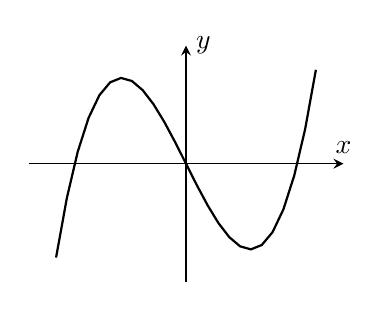
\begin{tikzpicture}[scale=1]
     \draw[->,>=stealth,semithick](-2,0)--(2,0)node[above]{$x$};%x軸
     \draw[->,>=stealth,semithick](0,-1.5)--(0,1.5)node[right]{$y$};%y軸
     \draw[thick,domain=-1.65:1.65] plot(\x,{pow(\x,3)-2*\x});
    \end{tikzpicture} 
  \end{minipage}
  \begin{minipage}[b]{0.45\linewidth}
   \begin{tikzpicture}[scale=1]
    \draw[->,>=stealth,semithick](-1,0)--(3,0)node[above]{$x$};%x軸
    \draw[->,>=stealth,semithick](0,-1.5)--(0,1.5)node[right]{$y$};%y軸
    \draw[thick,domain=-0.5:1] plot(\x,-1);
    \draw[thick,domain=1.06:2.5] plot(\x,1);
    \draw(1,1) circle [thick, radius=2pt];
    \fill(1,-1) circle [radius=2pt];
    \draw[dashed] (1,-1)--(1,0.94);
   \end{tikzpicture} 
  \end{minipage}
 \caption{連続関数と非連続関数}
 \label{fig:realcontinuous}
\end{figure}
\end{develop}



\section{同相写像}

\section{分離性}



\section{距離空間}







\end{document}